\newpage
\subsection{Μελέτη διαφορετικών Branch Predictors}
\vspace{3mm}

Στο σημείο αυτό μελετάμε την απόδοση διαφορετικών predicotrs στο σύνολο των
μετροπρογραμμάτων. Οι Predictors που συγκρίνονται είναι οι παρακάτω:

\begin{flushleft}
\begin{enumerate}[font=\small]
   \item Static Always Taken Predictor
   \item Static BTFNTPredictor (BackwardTaken-ForwardNotTaken)
   \item Nbit-8K-4bit 
   \item Pentium-M
   \item LocalHistory-PHT(8K, 2bit)-BHT(2K, 8bit)
   \item LocalHistory-PHT(8K, 2bit)-BHT(4K, 4bit)
   \item GlobalHistory-PHT(16K, 2bit)-BHR(5bit)
   \item GlobalHistory-PHT(8K, 4bit)-BHR(5bit)
   \item GlobalHistory-PHT(8K, 4bit)-BHR(10bit)
   \item GlobalHistory-PHT(16K, 2bit)-BHR(10bit)
   \item Tournament-1K-Entries
      \begin{itemize}
         \item $P_0$: Nbit-8K-2bit
         \item $P_1$: Nbit-4K-4bit
      \end{itemize}
   \item Tournament-2K-Entries
      \begin{itemize}
         \item $P_0$: GlobalHistory-PHT(4K, 4bit)-BHR(2bit)
         \item $P_1$: Nbit-8K-2bit
      \end{itemize}
   \item Tournament-1K-Entries
      \begin{itemize}
         \item $P_0$: GlobalHistory-PHT(8K, 2bit)-BHR(2bit)
         \item $P_1$: LocalHistory-PHT(2K, 4bit)-BHT(4K, 2bit)
      \end{itemize}
   \item Tournament-1K-Entries
      \begin{itemize}
         \item $P_0$: Nbit-8K-2bit
         \item $P_1$: GlobalHistory-PHT(8K, 2bit)-BHR(5bit)
      \end{itemize}
   \item Tournament-2K-Entries
      \begin{itemize}
         \item $P_0$: Nbit-8K-2bit
         \item $P_1$: GlobalHistory-PHT(8K, 2bit)-BHR(5bit)
      \end{itemize}
   \item Tournament-1K-Entries
      \begin{itemize}
         \item $P_0$: Nbit-2K-8
         \item $P_1$: LocalHistory-PHT(2K, 4bit)-BHT(4K, 2bit)
      \end{itemize}
   \item Alpha Predictor
\end{enumerate}
\end{flushleft}

\vspace{1em}    
Ακολουθούν τα διαγράμματα που προέκυψαν και ο σχετικός σχολιασμός
τους:
\vspace{1em}    

   \begin{minipage}{\textwidth}
      \begin{center}
         \fbox{\textlatin{\textbf{\textit{403-gcc}}}}\\
         \vspace{3mm}
         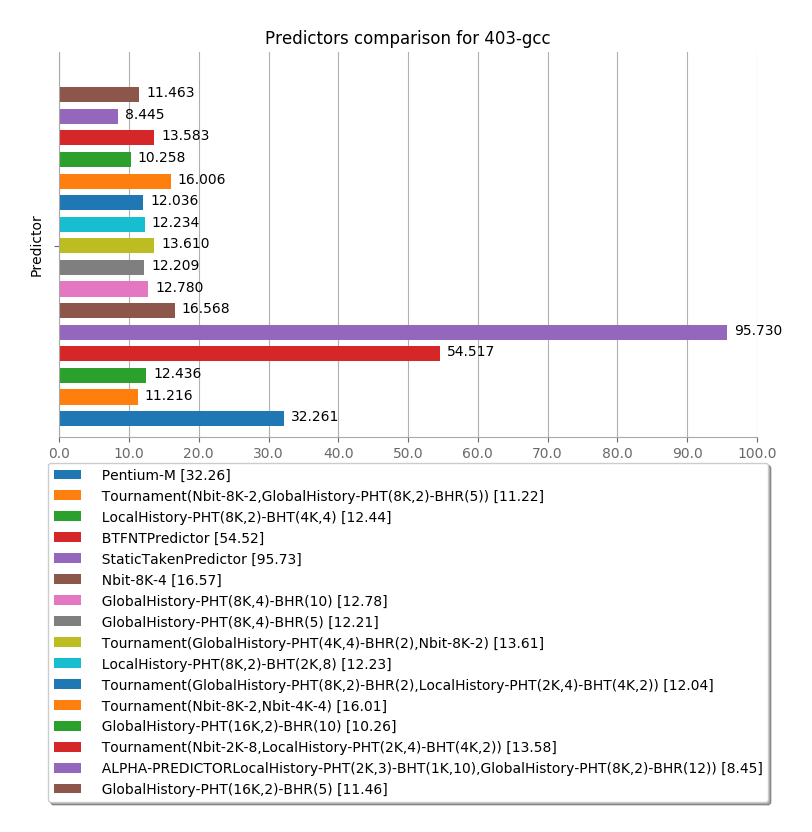
\includegraphics[width=0.9\textwidth, frame]{./graphs/4-5/403-gcc.png}
         \vspace{6mm}
      \end{center}
   \end{minipage}

   \begin{minipage}{\textwidth}
      \begin{center}
         \fbox{\textlatin{\textbf{\textit{429-mcf}}}}\\
         \vspace{3mm}
         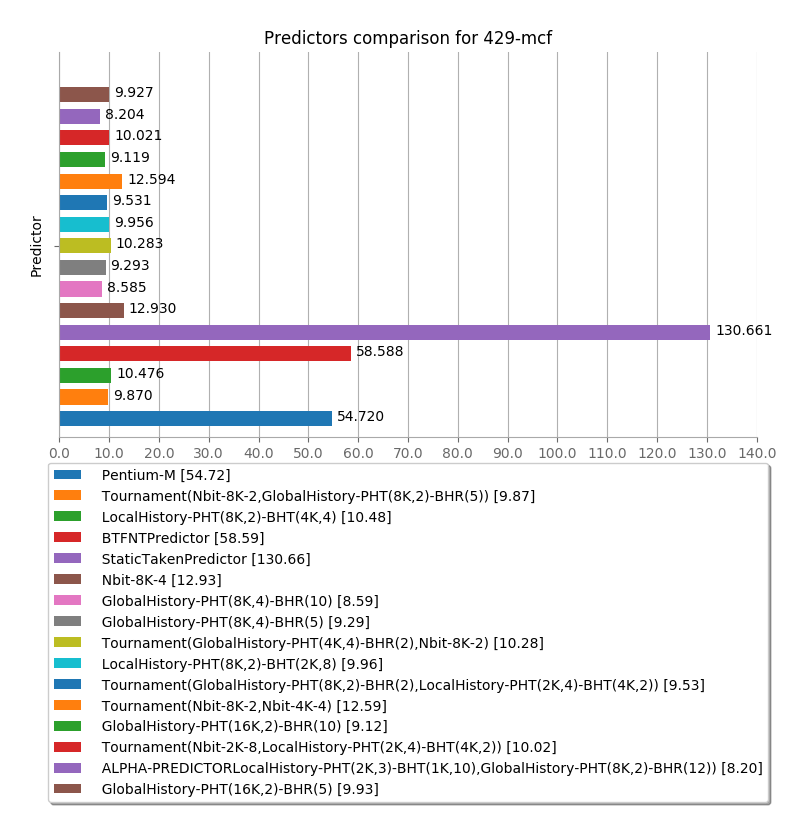
\includegraphics[width=0.9\textwidth, frame]{./graphs/4-5/429-mcf.png}
         \vspace{6mm}
      \end{center}
   \end{minipage}

   \begin{minipage}{\textwidth}
      \begin{center}
         \fbox{\textlatin{\textbf{\textit{434-zeusmp}}}}\\
         \vspace{3mm}
         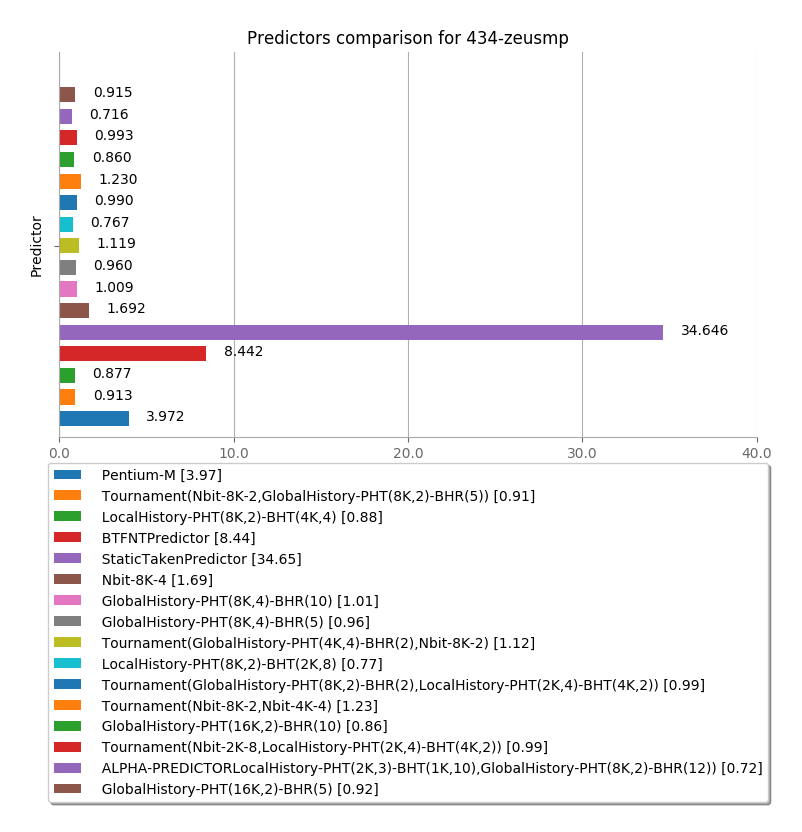
\includegraphics[width=0.9\textwidth, frame]{./graphs/4-5/434-zeusmp.png}
         \vspace{6mm}
      \end{center}
   \end{minipage}

   \begin{minipage}{\textwidth}
      \begin{center}
         \fbox{\textlatin{\textbf{\textit{436-cactusADM}}}}\\
         \vspace{3mm}
         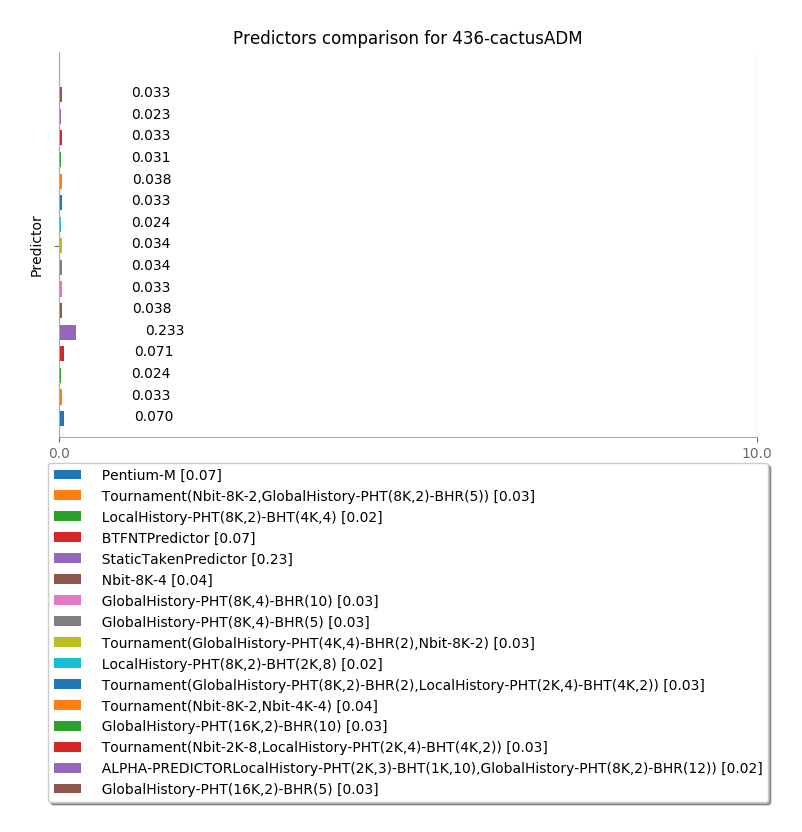
\includegraphics[width=0.9\textwidth, frame]{./graphs/4-5/436-cactusADM.png}
         \vspace{6mm}
      \end{center}
   \end{minipage}

   \begin{minipage}{\textwidth}
      \begin{center}
         \fbox{\textlatin{\textbf{\textit{445-gobmk}}}}\\
         \vspace{3mm}
         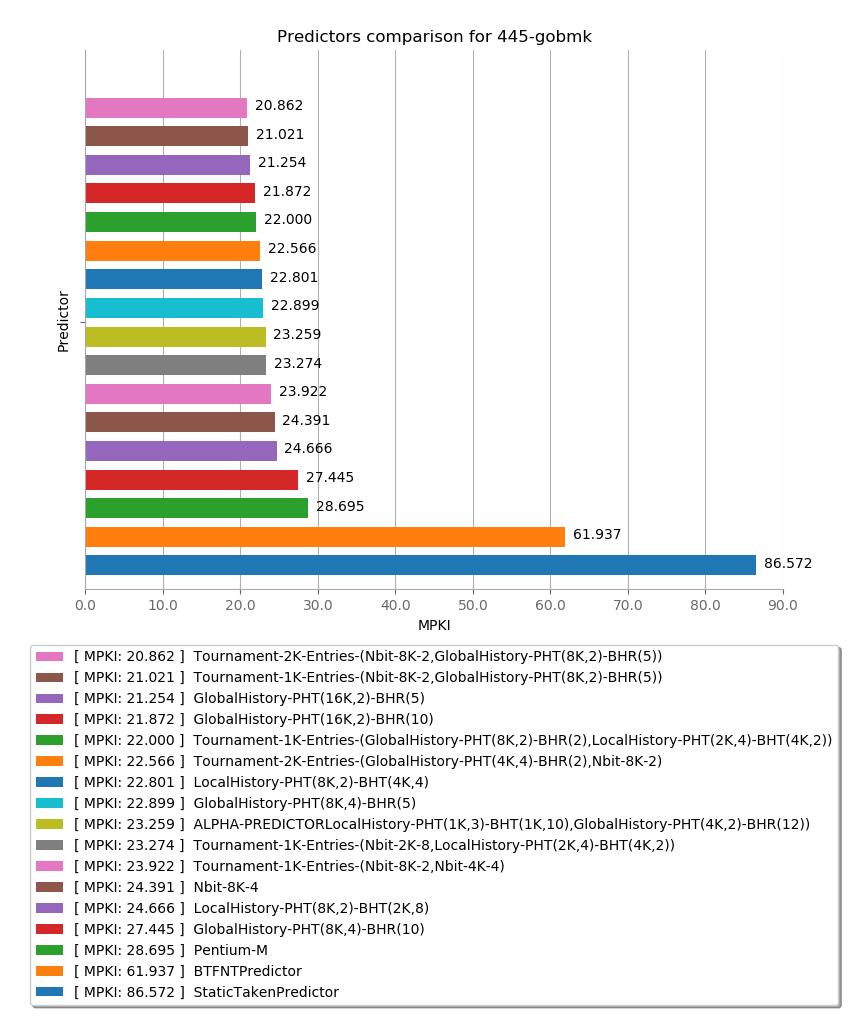
\includegraphics[width=0.9\textwidth, frame]{./graphs/4-5/445-gobmk.png}
         \vspace{6mm}
      \end{center}
   \end{minipage}

   \begin{minipage}{\textwidth}
      \begin{center}
         \fbox{\textlatin{\textbf{\textit{450-soplex}}}}\\
         \vspace{3mm}
         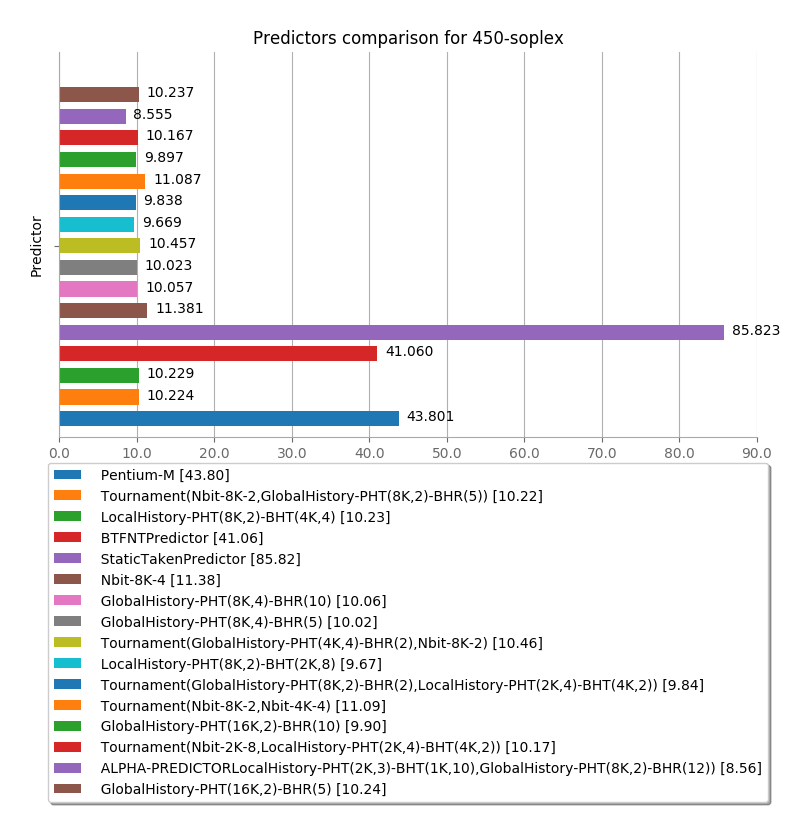
\includegraphics[width=0.9\textwidth, frame]{./graphs/4-5/450-soplex.png}
         \vspace{6mm}
      \end{center}
   \end{minipage}

   \begin{minipage}{\textwidth}
      \begin{center}
         \fbox{\textlatin{\textbf{\textit{456-hmmer}}}}\\
         \vspace{3mm}
         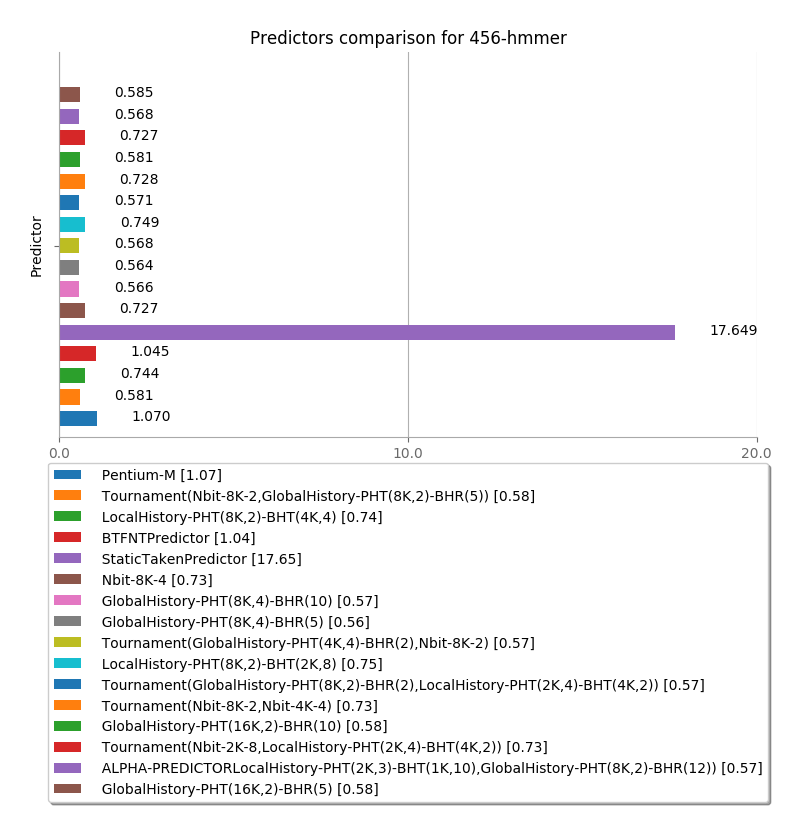
\includegraphics[width=0.9\textwidth, frame]{./graphs/4-5/456-hmmer.png}
         \vspace{6mm}
      \end{center}
   \end{minipage}

   \begin{minipage}{\textwidth}
      \begin{center}
         \fbox{\textlatin{\textbf{\textit{458-sjeng}}}}\\
         \vspace{3mm}
         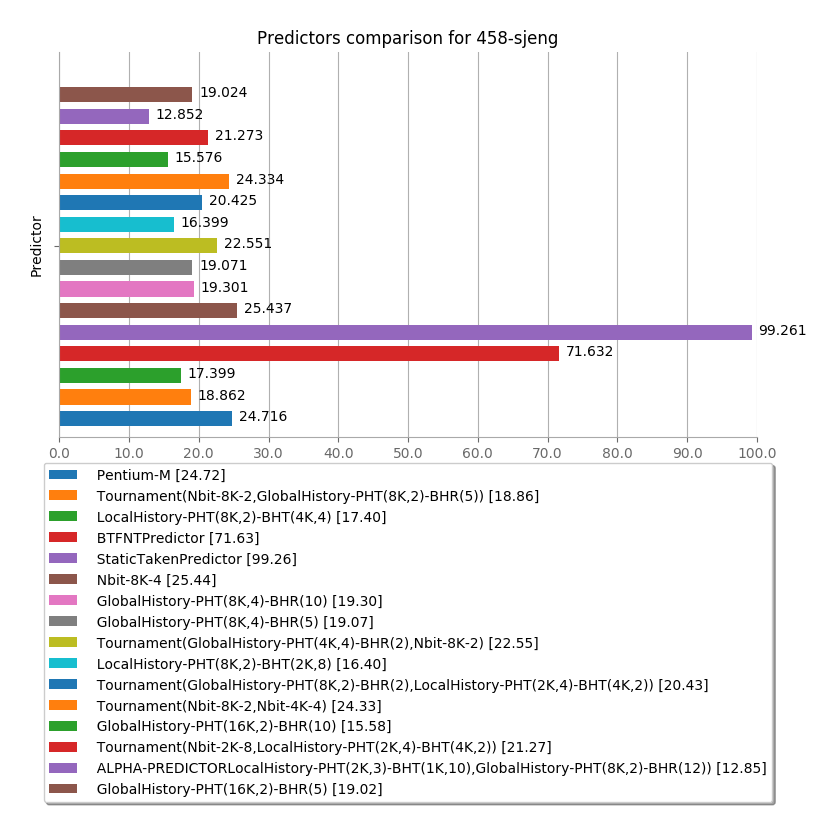
\includegraphics[width=0.9\textwidth, frame]{./graphs/4-5/458-sjeng.png}
         \vspace{6mm}
      \end{center}
   \end{minipage}

   \begin{minipage}{\textwidth}
      \begin{center}
         \fbox{\textlatin{\textbf{\textit{459-GemsFDTD}}}}\\
         \vspace{3mm}
         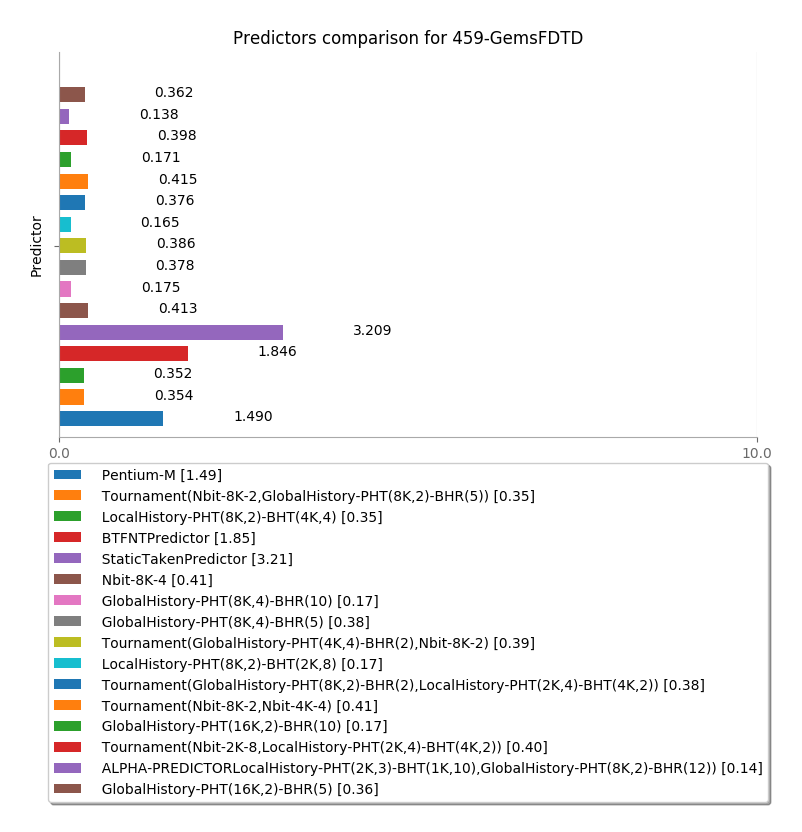
\includegraphics[width=0.9\textwidth, frame]{./graphs/4-5/459-GemsFDTD.png}
         \vspace{6mm}
      \end{center}
   \end{minipage}

   \begin{minipage}{\textwidth}
      \begin{center}
         \fbox{\textlatin{\textbf{\textit{471-omnetpp}}}}\\
         \vspace{3mm}
         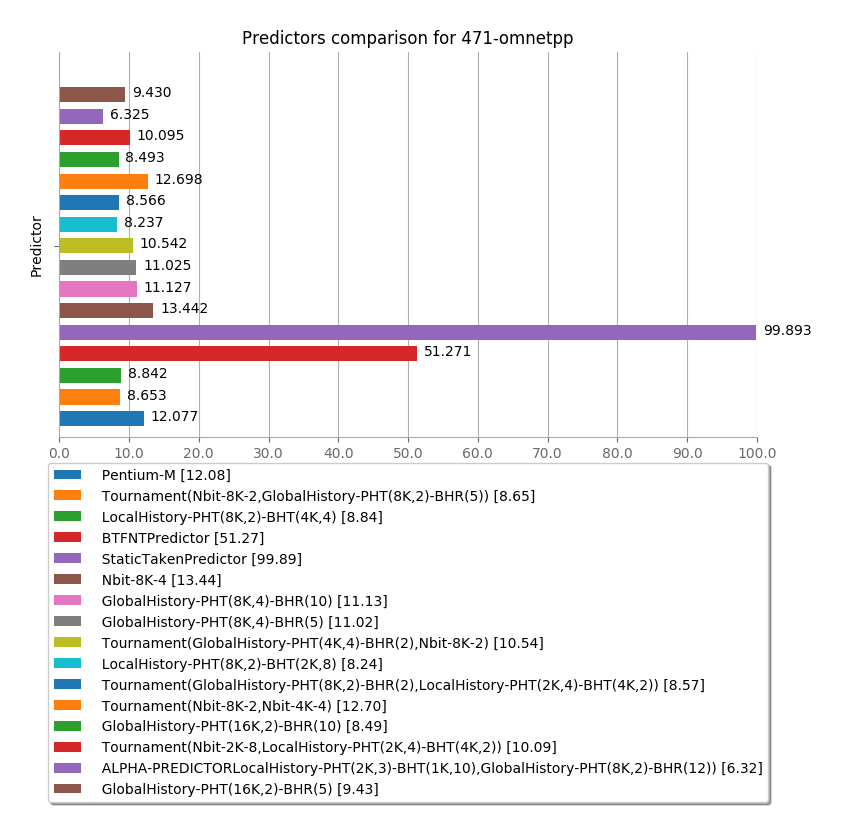
\includegraphics[width=0.9\textwidth, frame]{./graphs/4-5/471-omnetpp.png}
         \vspace{6mm}
      \end{center}
   \end{minipage}

   \begin{minipage}{\textwidth}
      \begin{center}
         \fbox{\textlatin{\textbf{\textit{473-astar}}}}\\
         \vspace{3mm}
         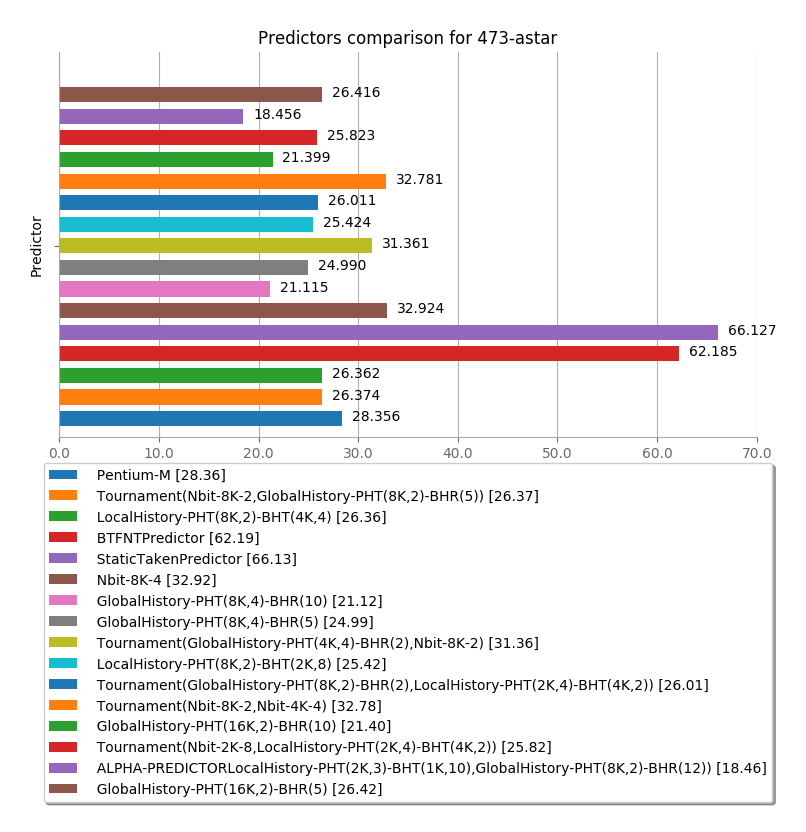
\includegraphics[width=0.9\textwidth, frame]{./graphs/4-5/473-astar.png}
         \vspace{6mm}
      \end{center}
   \end{minipage}

   \begin{minipage}{\textwidth}
      \begin{center}
         \fbox{\textlatin{\textbf{\textit{483-xalancbmk}}}}\\
         \vspace{3mm}
         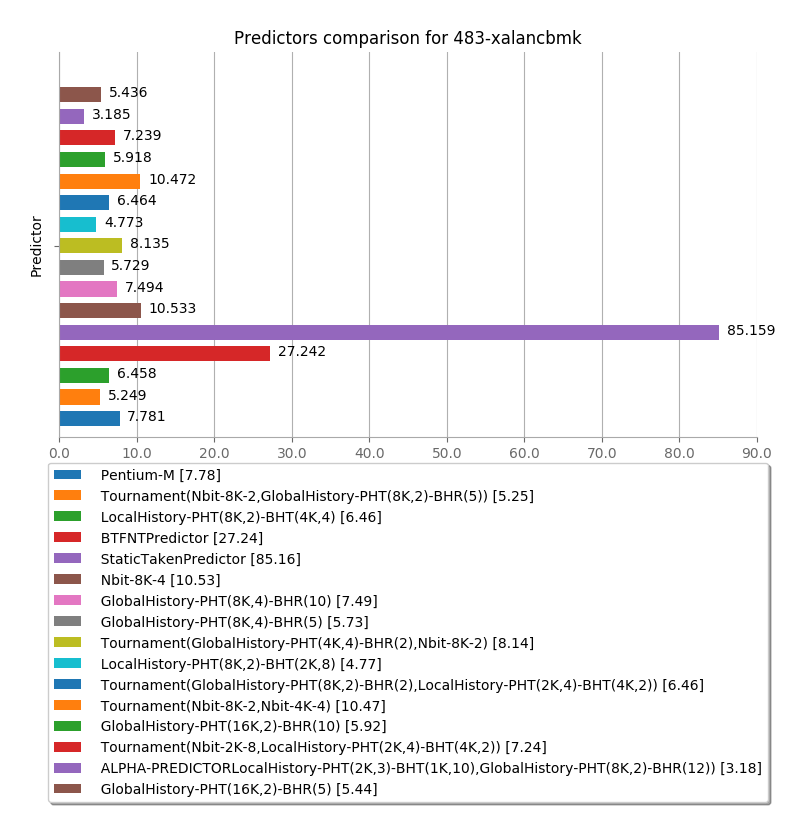
\includegraphics[width=0.9\textwidth, frame]{./graphs/4-5/483-xalancbmk.png}
         \vspace{6mm}
      \end{center}
   \end{minipage}


   \begin{minipage}{\textwidth}
      \begin{center}
         \fbox{\textlatin{\textbf{\textit{Geometric Average of MPKI}}}}\\
         \vspace{3mm}
         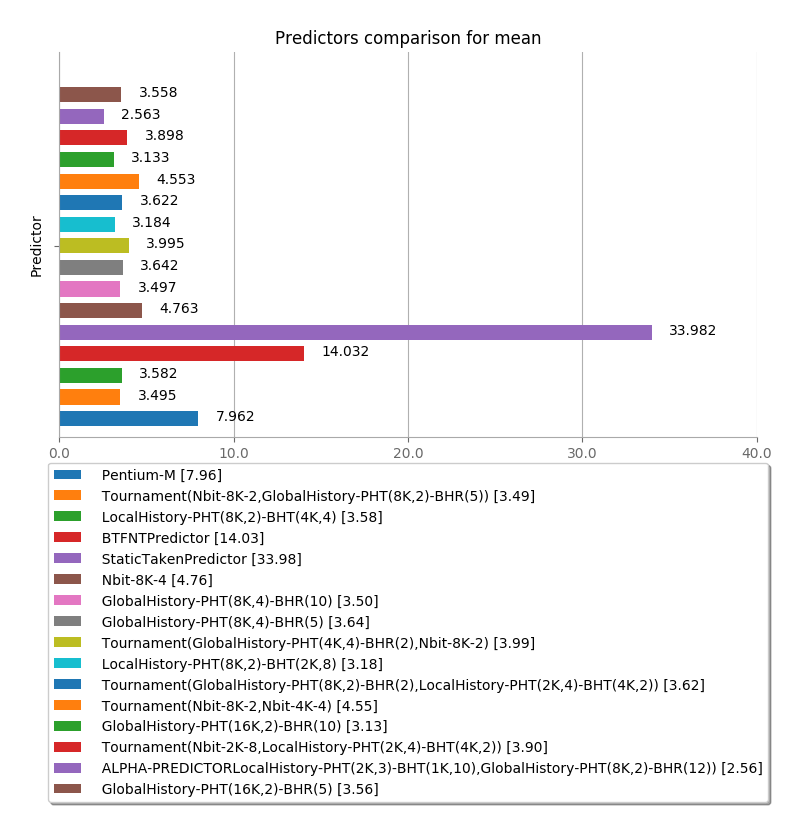
\includegraphics[width=0.9\textwidth, frame]{./graphs/4-5/mean.png}
         \vspace{6mm}
      \end{center}
   \end{minipage}
\newpage
\paragraph{Συμπεράσματα-Σχόλια}
   Όπως είναι αναμενόμενο, ο Static Always Taken Predictor έχει τη χειρότερη
   επίδοση σε όλα τα μετροπρογράμματα. Επόμενος χειρότερος predictor είναι ο
   BTFNT, εξίσου αναμενόμενο αφού πρόκειται για static predictor, με ελαφρά
   ωστόσο καλύτερη επίδοση από τον Always Taken. Ακολουθεί ο Pentium Predictor. 
  
   Όσον αφορά την επιλογή ενός συγκεκριμένουν predictor, θα πρέπει να λάβουμε
   υπ' όψιν την χρήση που θα κάνει το σύστημα. Αν το προφίλ της χρήσης κάνει
   align με ένα ή περισσότερα benchmarks τότε θα διαλέξουμε τον predictor που τα
   πηγαίνει καλύτερα σε αυτήν την χρήση. Επειδή στη μελέτη αυτή όμως δε δίνεται
   έμφαση σε ένα συγκεκριμένο benchmark, θα κρίνουμε με βάση τη συνολική επίδοση
   των 12 προγηούμενων benchmarks κατά μέσο όρο. Για τη συνολική αυτή εποπτεία,
   παραθέτουμε το τελευταίο διάγραμμα, των γεωμετρικών μέσων όρων. Με βάση το
   διάγραμμα αυτό, και επιβεβαιώνοντας από τα επιμέρους διαγράμματα των
   benchmarks, συμπεραίνουμε πως ο \textbf{Alpha Predictor} έχει κατά μέσο όρο
   την καλύτερη επίδοση (χαμηλό MPKI) συνολικά, αλλά και την καλύτερη επίδοση σε
   κάθε ένα από τα benchmarks. Εξίσου καλά ωστόσο αποδίδουν και οι
   GlobalHistory-PHT(16K, 2bit)-BHR(10bit) LocalHistory-PHT(8K, 2bit)-BHT(2K,
   8bit).

   \vspace{1em}
   \noindent Συνολικά, με βάση τις γεωμετρικές μέσες τιμές, οι predictors σε σειρά
   φθίνουσας επίδοσης είναι: {\small 
   \begin{enumerate}
      \item Alpha Predictor
      \item GlobalHistory-PHT(16K, 2bit)-BHR(10bit)
      \item LocalHistory-PHT(8K, 2bit)-BHT(2K, 8)
      \item Tournament-2K-Entries-(Nbit-8K-2, GlobalHistory-PHT(8K, 2bit)-BHR(5bit))
      \item Tournament-1K-Entries-(Nbit-8K-2, GlobalHistory-PHT(8K, 2bit)-BHR(5bit))
      \item GlobalHistory-PHT(8K, 4bit)-BHR(10bit)
      \item GlobalHistory-PHT(16K, 2bit)-BHR(5bit)
      \item LocalHistory-PHT(8K, 2bit)-BHT(4K, 4bit)
      \item Tournament-1K-Entries-(GlobalHistory-PHT(8K, 2bit)-BHR(2bit), LocalHistory-PHT(2K, 4bit)-BHT(4K, 2bit))
      \item GlobalHistory-PHT(8K, 4bit)-BHR(5bit)
      \item Tournament-1K-Entries-(Nbit-2K-8, LocalHistory-PHT(2K, 4bit)-BHT(4K, 2bit))
      \item Tournament-2K-Entries-(GlobalHistory-PHT(4K, 4bit)-BHR(2bit), Nbit-8K-2bit)
      \item Tournament-1K-Entries-(Nbit-8K-2, Nbit-4K-4bit)
      \item Nbit-8K-4bit
      \item Pentium-M
      \item BTFNTPredictor
      \item StaticTakenPredictor
   \end{enumerate}
   }
   \vspace{1em}
   \noindent \textbf{Άρα, θα επέλεγα για συνολικά καλύτερη επίδοση, τoν Alpha Predictor.}